\documentclass[12pt]{article}

\usepackage{sbc-template}
\usepackage{graphicx,url}
\usepackage[utf8]{inputenc}
\usepackage[brazil]{babel}

\sloppy

\title{Sistema de Apoio à Decisão para Segurança em Redes IoT com Aprendizado de Máquina}

\author{Antônio Marcos\inst{1}}

\address{Departamento de Ciência da Computação -- Universidade Federal de Juiz de Fora (UFJF)\\
  Juiz de Fora -- MG -- Brazil
  \email{antoniomarcos.souza2002@gmail.com}
}

\begin{document}

\maketitle

\begin{abstract}
  Redes de dispositivos IoT expandem a superfície de ataque e exigem mecanismos que apoiem administradores na identificação e priorização de ameaças.
  Este trabalho propõe um Sistema de Apoio à Decisão (SAD) que combina classificação de tráfego, explicabilidade e regras operacionais sobre o dataset CIC-IoT-2023.
  O pipeline reproduzível integra pré-processamento, seleção de atributos, comparação de estratégias de balanceamento, otimização de hiperparâmetros com Optuna e rastreamento com MLflow.
  Um dashboard estilo SOC consome modelos treinados offline para inferência, monitoramento simulado, alertas, explicações SHAP e análise de sensibilidade de limiares.
  Os resultados indicam que a abordagem transforma previsões em recomendações acionáveis para analistas de segurança.
\end{abstract}

\begin{resumo}
  A segurança em redes IoT requer apoio sistemático à decisão além da detecção isolada de intrusões.
  Desenvolvemos um SAD com pipeline de ML reproduzível, explicabilidade e dashboard operacional baseado no CIC-IoT-2023.
  O sistema prioriza ameaças, gera recomendações e permite simular cenários de decisão sem retreinar modelos em produção.
\end{resumo}

\section{Introdução}

A proliferação de dispositivos IoT amplia vetores de ataque como DDoS, varreduras e malware botnet.
Administradores de rede precisam não apenas detectar eventos maliciosos, mas decidir rapidamente entre monitorar, investigar ou isolar ativos.

A pergunta-problema deste trabalho é: \textit{como apoiar a tomada de decisão de administradores de redes IoT na identificação, monitoramento e priorização de ameaças utilizando modelos de aprendizado de máquina?}

Contribuímos com: (i) pipeline modular e reproduzível; (ii) comparação de balanceamento e modelos; (iii) explicabilidade com SHAP; (iv) motor de regras de apoio à decisão; (v) demonstração operacional via dashboard.

\section{Metodologia}

\subsection{Dataset e pré-processamento}

Utilizamos o dataset CIC-IoT-2023, com tráfego rotulado em dezenas de tipos de ataque.
Aplicamos amostragem estratificada de 1\% dos 62 arquivos CSV, normalização de rótulos e mapeamento para tarefa binária (BENIGN vs ATTACK) e multiclasse em oito grupos (DDoS, DoS, Mirai, Recon, Spoofing, Web, BruteForce, Benign).

O pré-processamento remove duplicatas, valores inválidos e colunas de variância zero, aplica \textit{StandardScaler} e divide os dados em treino, validação e teste de forma estratificada (seed fixa).

\subsection{Engenharia de atributos}

Features altamente correlacionadas ($|r| > 0{,}9$) são removidas.
Mutual information e importância de Random Forest orientam a seleção final, documentada em artefatos versionados.

\subsection{Modelos e balanceamento}

Avaliamos Regressão Logística, Random Forest, XGBoost e LightGBM com pipeline compartilhado.
Comparamos três estratégias de desbalanceamento: sem tratamento, \textit{class weights} e SMOTE.
Hiperparâmetros de RF, XGBoost e LightGBM são otimizados com Optuna maximizando F1 macro.
Experimentos são registrados no MLflow (métricas, parâmetros, matrizes e curvas).

\subsection{Sistema de apoio à decisão}

Scores de risco derivam das probabilidades de ataque e são classificados em níveis Baixo, Médio, Alto e Crítico.
Um motor de regras traduz níveis em ações: bloqueio e isolamento (crítico), investigação (alto) ou monitoramento contínuo (médio).
O dashboard Streamlit simula tráfego em tempo real, exibe alertas, explicações SHAP e análise what-if de limiares --- sem treinamento online.

\section{Resultados}

A Tabela~\ref{tab:metrics} resume métricas do melhor modelo selecionado no conjunto de teste.
O sistema registra accuracy, precision, recall, F1, ROC-AUC e PR-AUC, além de matrizes de confusão e curvas ROC/PR como artefatos.

\begin{table}[ht]
\centering
\caption{Métricas do melhor modelo (LightGBM) no conjunto de teste}
\label{tab:metrics}
\begin{tabular}{lcccccc}
\hline
Modelo & Acc. & Prec. & Rec. & F1 & ROC-AUC & PR-AUC \\
\hline
LightGBM & 0.988 & 0.912 & 0.919 & 0.915 & 0.997 & 0.904 \\
\hline
\end{tabular}
\end{table}

A comparação de balanceamento e tuning indica trade-offs entre recall de ataques e falsos positivos, informando a escolha de limiares na página de simulação de cenários.

\begin{figure}[ht]
\centering
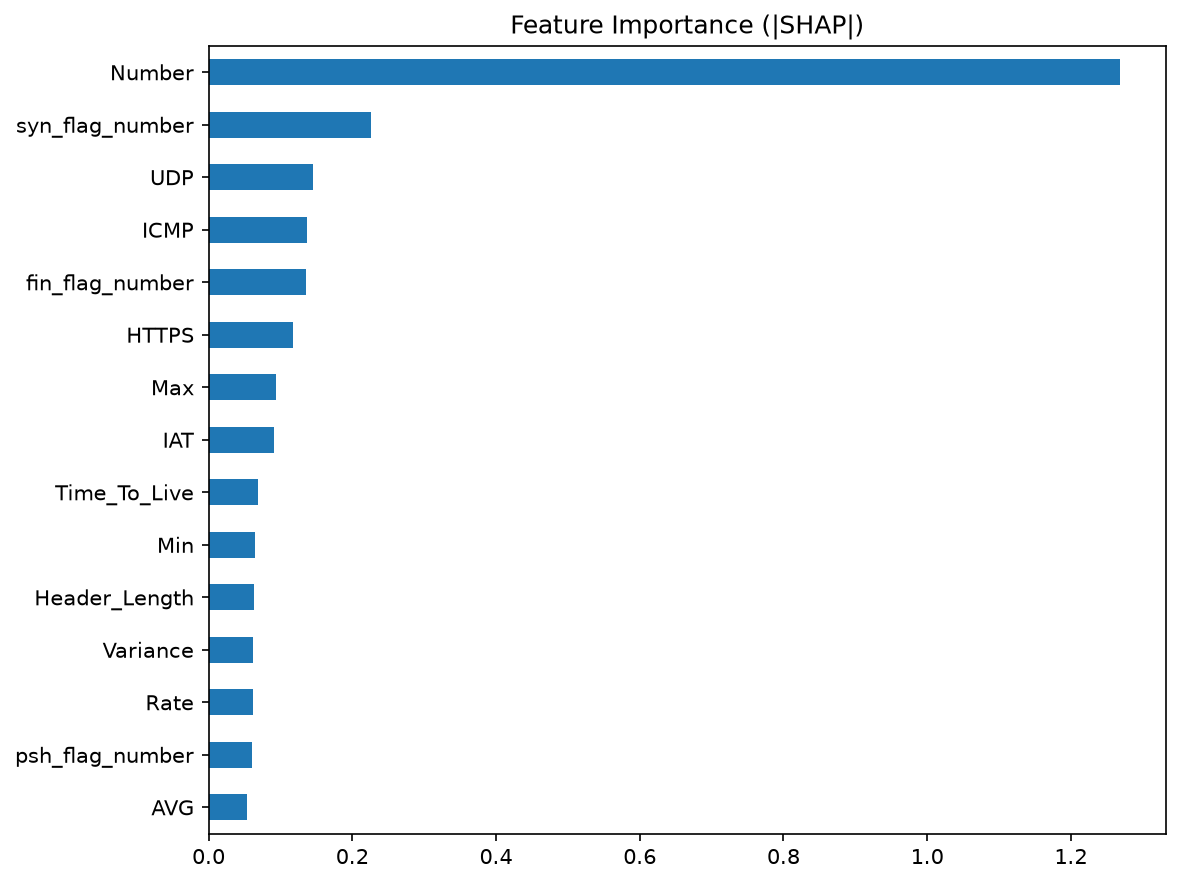
\includegraphics[width=.75\textwidth]{../reports/shap/feature_importance.png}
\caption{Importância de atributos via valores SHAP (gerada pelo pipeline).}
\label{fig:shap}
\end{figure}

\section{Discussão}

A arquitetura separa ML offline da operação online, alinhando-se a práticas de MLOps e ao escopo de SAD: decisões derivadas de evidências quantitativas e explicáveis.
Limitações incluem dependência de dados históricos, custo computacional do dataset completo e generalização para novos vetores de ataque.
A análise de sensibilidade de limiares explicita o compromisso entre detecção e alarmes falsos --- central para administradores.

\section{Conclusão}

Apresentamos um SAD para segurança IoT que integra detecção por ML, explicabilidade e recomendações operacionais.
O protótipo demonstra monitoramento simulado e apoio à decisão em ambiente estilo SOC, indo além de um classificador isolado.
Trabalhos futuros incluem integração com SIEM real, detecção de \textit{drift} e validação em redes de produção.

\bibliographystyle{sbc}
\bibliography{sbc-template}

\end{document}
